\Askhsh{18550}{2}
\begin{ylh}{1}
    \item 7.4. Ανάλογα ευθύγραμμα τμήματα - Αναλογίες
    \item 10.3. Εμβαδόν βασικών ευθύγραμμων σχημάτων.
\end{ylh}
\begin{wrapfigure}[9]{r}{5cm}
\centering
\begin{tikzpicture}[scale=0.75]
    % Ορισμός κορυφών ορθογωνίου (Α, Β, Γ, Δ)
    % Υποθέτουμε x=4, y=8, z=6 για τη σχεδίαση
    \tkzDefPoint(0,0){A}
    \tkzDefPoint(12,0){B} % x+y = 4+8 = 12
    \tkzDefPoint(12,6){G} % Γ (Gamma)
    \tkzDefPoint(0,6){D} % Δ (Delta)
    
    % Ορισμός σημείου Ε στην πλευρά ΑΒ
    \tkzDefPoint(4,0){E} % AE = x = 4
    
    % Σχεδίαση του ορθογωνίου
    \tkzDrawPolygon[line width=0.8pt, draw=black](A,B,G,D)
    
    % Σχεδίαση των τμημάτων ΔΕ και ΓΕ
    \tkzDrawSegments[line width=0.8pt, draw=black](D,E E,G)
    
    % Ετικέτες σημείων
    \tkzLabelPoint[below left](A){A}
    \tkzLabelPoint[below right](B){B}
    \tkzLabelPoint[above right](G){$\Gamma$}
    \tkzLabelPoint[above left](D){$\Delta$}
    \tkzLabelPoint[below](E){E}
    
    % Ετικέτες μηκών
    \tkzLabelSegment[below](A,E){$x$}
    \tkzLabelSegment[below](E,B){$y$}
    \tkzLabelSegment[right](B,G){$z$}
\end{tikzpicture}
\end{wrapfigure}
Η περίμετρος του ορθογωνίου ΑΒΓΔ του σχήματος είναι 36 και το Ε είναι σημείο στην πλευρά ΑΒ. Τα μήκη των τμημάτων $x$, $y$, $z$ είναι ανάλογα προς τους αριθμούς $2,4,3$ αντίστοιχα.
\begin{alist}
\item Να αποδείξετε ότι $x = 4$, $y = 8$ και $z = 6$. \monades{13}
\item 
    \begin{rlist}
    \item Να υπολογίσετε το εμβαδόν του τριγώνου ΓΕΔ.
    \item Να βρεθεί ο λόγος του εμβαδού του τριγώνου ΓΔΕ προς το εμβαδόν του ορθογωνίου ΑΒΓΔ. \monades{12}
    \end{rlist}
\end{alist}